\section{Results}
\label{sec:results}

\subsection{Two matched-budget repairs}
\label{sec:repairs}
Table~\ref{tab:repair-summary} summarizes two diagnosis-guided repairs
at matched budgets: covariance initialization improves two-call
CIFAR-10 generation, and ordinary continuation corrects MNIST
overrepresentation at equal updates. Coverage uses an ordinary paired
95\% interval; largest-region entries are pooled masses, with teacher
mass 0.3535.

\begin{table}[t]
\centering
\caption{Matched-budget outcomes for the two repairs: control, repair,
paired difference $\Delta$, and its interval $[\ell,u]$ (Sec.~\ref{sec:metrics}).}
\label{tab:repair-summary}
\footnotesize
\setlength{\tabcolsep}{3pt}
\sisetup{group-digits=false, retain-explicit-plus}
\begin{tabular}{@{}l
  S[table-format=+1.5]
  S[table-format=+1.4]
  S[table-format=1.4]@{}}
\toprule
\multicolumn{4}{@{}l}{\emph{CIFAR-10, two denoiser calls}} \\
\addlinespace[1pt]
 & {KID $\downarrow$} & {Coverage $\uparrow$} & {Largest region} \\
\cmidrule(l){2-4}
Control      & 0.1858   & 0.206   & 0.9730 \\
Repair       & 0.1264   & 0.288   & 0.9129 \\
$\Delta$     & -0.05938 & +0.0821 & {--} \\
$[\ell,u]$   & \multicolumn{1}{c}{\scriptsize$[-0.06138,-0.05739]$} & \multicolumn{1}{c}{\scriptsize$[0.0672,0.0970]$} & \\
\midrule
\multicolumn{4}{@{}l}{\emph{MNIST, 8,000 updates}} \\
\addlinespace[1pt]
 & {Class-mass error $\downarrow$} & {Digit-3 error $\downarrow$} & \\
\cmidrule(l){2-3}
Control      & 0.02177  & 0.06837 & \\
Repair       & 0.00900  & 0.00747 & \\
$\Delta$     & -0.01277 & -0.06090 & \\
$[\ell,u]$   & \multicolumn{1}{c}{\scriptsize$[-0.01878,-0.00676]$} & \multicolumn{1}{c}{\scriptsize$[-0.11814,-0.00366]$} & \\
\bottomrule
\end{tabular}
\end{table}

\subsection{Covariance start improves two-call KID and coverage}
\label{sec:cifar}
The covariance start reduces two-call KID by 32.0\% and raises real-data
coverage from 0.206 to 0.288 (Fig.~\ref{fig:cifar_initializer}), achieving
the lowest KID among same-budget arms. Full-moment initialization gives
coverage 0.290 and KID 0.1405; DPM++ and UniPC both give KID 0.2225.
The frozen selector first chose full-moment initialization
(Sec.~\ref{sec:policy}). Its paired-seed ablation isolated covariance as
the active component, and the separate six-arm study confirmed the
covariance start on fresh samples.

\begin{figure}[t]
\centering
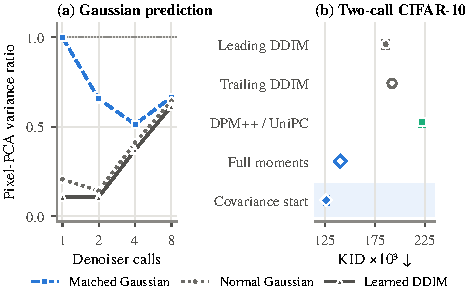
\includegraphics[width=\linewidth]{../figures/initialization_repair.pdf}
\caption{Correcting the initial covariance improves two-call generation.
(a) Fresh confirmation over five generated-sample panels; whiskers are
95\% intervals. (b) Gaussian predictions and learned DDIM in a common
teacher-fit pixel basis separate initialization from integration.}
\label{fig:cifar_initializer}
\end{figure}

\Cref{eq:gaussian} predicts the useful regime: standard-normal-to-matched
aggregate variance ratios are 0.216, 0.800, and 0.968 at two, four, and
eight calls. Learned trajectories correlate with the Gaussian prediction
at four/eight calls (Spearman 0.938/0.894). At these larger budgets,
full-moment initialization gives KID 0.0926/0.0378 versus DDIM's
0.0903/0.0363 (Supp.~Secs.~D--F), concentrating the benefit at the
smallest budget.

The repair improves real-data discrepancy and coverage. Concentration in
the largest teacher region falls from 97.30\% to 91.29\%, while the
fraction within the real-training 1--99\% frequency range rises from
0.72\% to 24.7\%. Evaluating the same outputs against CIFAR-10.1v6 lowers
KID from 0.19060 to 0.12832 (32.7\%) and raises coverage from 0.3221 to
0.4268. The paired KID difference is $-0.06228$
[$-0.06422,-0.06035$], with 95\% simultaneous coverage across four
contrasts (Supp.~Sec.~F.4). Supp.~Sec.~N.1 reports the remaining
teacher-relative deficit and precision change.

\subsection{Intervention location separates spread from useful coverage}
\label{sec:numerical}
At four calls, output covariance restoration raises pixel spread from
0.376 to 0.917, yet coverage falls from 0.478 to 0.332 and KID rises
from 0.0903 to 0.1024 (Fig.~\ref{fig:numerical_repair}). UniPC instead
reaches coverage 0.549 and KID 0.0694. At eight calls, output restoration
again raises KID (0.0363 to 0.0505), while UniPC reaches 0.0245
(Supp.~Sec.~F.2). The audit distinguishes restored spread from improved
real-data coverage.
\begin{figure}[t]
\centering
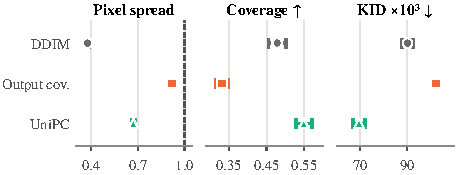
\includegraphics[width=\linewidth]{../figures/numerical_repair.pdf}
\caption{Restoring output spread can degrade useful coverage (four-call
CIFAR-10, five paired panels). Pixel spread is teacher-relative; coverage
and KID use real data.}
\label{fig:numerical_repair}
\end{figure}
The same discipline transfers to a second, independently pretrained
checkpoint (Fig.~\ref{fig:edm_solver_audit}). On the EDM model, Heun lowers
KID from 0.00876 to 0.00250 at 15 calls and from Euler's 0.00250 to
0.000413 at 35 calls, with coverage 0.501 for both solvers at 35 calls.
At 15 calls the audit also exposes a coverage trade-off that KID alone
hides, from 0.477 to 0.417. Small-budget behaviour and the frequency check
are in Supp.~Sec.~N.2.

\begin{figure}[t]
\centering
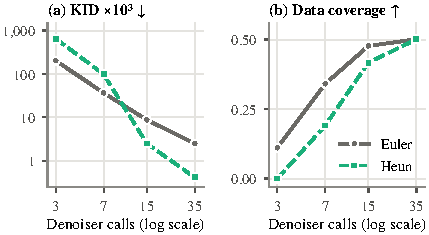
\includegraphics[width=\linewidth]{../figures/edm_solver_audit.pdf}
\caption{EDM solver choice changes with budget. Points are descriptive,
without model-seed uncertainty.}
\label{fig:edm_solver_audit}
\end{figure}

\subsection{Signed mass measurements enable calibrated semantic repair}
\label{sec:mnist}
Signed mass measurements reveal an overcorrection that a depletion test
cannot see, and ordinary continuation repairs it. They distinguish missing
probability from excess probability (Supp.~Sec.~H.2). Withholding digit~3
creates persistent real-data-relative depletion under DDIM25, DDIM50, and
DPM++25 in all three training seeds. At DPM++25, ordinary restoration
raises digit-3 mass from 0.00087 to 0.08747, toward the data target
0.0983; the adjusted paired increase is 0.08660 [0.07677,0.09643].
Coverage rises from 0.727 to 0.777, and the declared
five-percentage-point fidelity margins pass against the full-data control.
Doubling the restored digit's training weight overshoots to mass 0.1618. At equal updates, ordinary continuation reduces class-mass error by
58.7\% and digit-3 error by 89.1\% (Table~\ref{tab:repair-summary}).
The ordinary and targeted branches assign 9.08\% and 16.67\% of outcomes
to digit~3, against the real reference's 9.83\%. All four precision and
consensus fidelity constraints pass, and acceptance matches the full-data
control. Both error reductions also hold under DDIM25/DDIM50; digit-3
equivalence within $\pm0.03$ holds in all nine ordinary-continuation
seed--sampler probes. Diagnosis costs 48,000 images and 1.6 million
denoiser calls per checkpoint (Supp.~Sec.~H.2).
\begin{figure}[t]
\centering
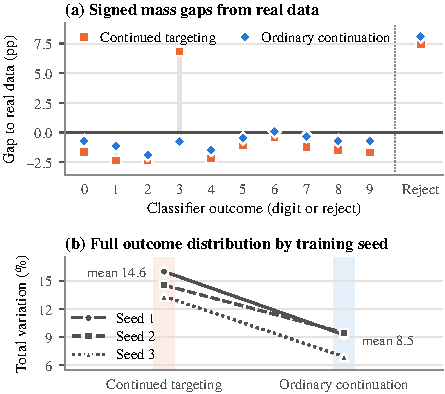
\includegraphics[width=\linewidth]{../figures/mnist_full_balance.pdf}
\caption{Ordinary continuation reduces imbalance across all classifier
outcomes, including rejection. (a) Mean signed gaps to real data.
(b) Total variation per training seed at 8,000 updates.}
\label{fig:mnist-full-balance}
\end{figure}
Across all eleven classifier outcomes, including rejection, total
variation falls from 0.1461 to 0.0854 (41.6\%), with descriptive paired
difference $-0.0608$ [$-0.0828,-0.0387$]
(Fig.~\ref{fig:mnist-full-balance}). Improvement holds in all three seeds.
On CIFAR-10 semantic regions, ordinary continuation improves DPM25 KID
from 0.01479 to 0.01010 and ten-region mass error from 0.0247 to 0.0148.
Both improve under all five samplers, fidelity constraints pass, and both
outperform event-ratio weighting under all three long-step probes.
Reference refinement and further controls appear in Supp.~Sec.~N.3.

\subsection{Crossed probes separate sampler deficits from persistent depletion}
\label{sec:crossed-probes}
Crossed probes distinguish deficits responsive to longer sampling from
depletion persisting across qualified samplers. All 12 short-sampler
cases from withheld training states retained digit-3 depletion under
three resolved probes and received sampler and training recommendations.
The other 18 received a sampler test; an occupancy-only rule would send
nine to retraining. On fresh samples, longer sampling improves
class-mass error, coverage, and acceptance in all 18. For persistent
cases, ordinary restoration with the resolved sampler raises digit-3
mass to 0.08567 versus 0.00067 under continued withholding at equal
updates. Cost and remaining contrasts appear in Supp.~Sec.~N.4.

\subsection{Conditioning and reference matching resolve diversity reversals}
\label{sec:t2i}
Exploratory comparisons show that pooling and teacher choice can reverse
the measured direction of diversity. DDIM4 has pooled DINO spread ratio
0.919 [0.910,0.928] but within-prompt ratio 1.306 [1.236,1.382]
(Fig.~\ref{fig:t2i_representations}). Within-prompt variation rises from
0.400 to 0.523 of reference pooled spread, while the between-prompt
component falls from 0.600 to 0.396, bringing the sum below one.
Sampling-latent and image-re-encoding ratios are 0.414 and 0.482; the
increased feature spread accompanies lower learned preference
(Supp.~Sec.~N.5).
\begin{figure}[t]
\centering
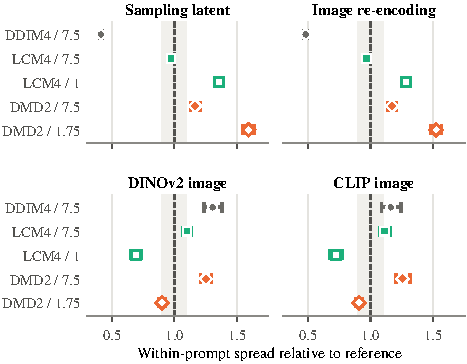
\includegraphics[width=\linewidth]{../figures/t2i_representation_reference.pdf}
\caption{Conditioning and reference matching change the measured direction
of within-prompt spread (descriptive intervals). Rows give sampler and teacher CFG; open markers
use the alternate teacher. The band marks $[0.9,1.1]$.}
\label{fig:t2i_representations}
\end{figure}
Matching the teacher changes the conclusion about a distilled model. DMD2's
DINO ratio moves from 1.251 [1.208,1.297] against CFG7.5 to
0.901 [0.873,0.929] against its matched CFG1.75 teacher; against that
teacher, latent spread increases to 1.592 and learned preference reaches
0.558 [0.545,0.571]. Sana Euler8 reduces latent spread to 0.763
[0.746,0.779] while DINO spread rises to 1.118 [1.083,1.157]. At eight
calls, Flow-DPM++ retains paired learned preference within tolerance,
0.479 [0.471,0.487]. CADS increases DINO spread to 1.965 [1.828,2.121] but
lowers preference to 0.354 [0.339,0.369].

\subsection{Validation makes the diagnostic resolution explicit}
\label{sec:supportcontrols}
Controlled deletions confirm that the audit resolves the deficits it is
designed to find, including ones that marginal and projected tests miss.
Removing one joint Gaussian component while retaining all marginal modes
is detected in 200/200 trials at 1,000 samples per set. NDB also detects
every joint removal, while both projected rules detect 0/200. Combined
removal, contraction, and translation produce all three labels in 200/200
trials. Rotation yields support departure in 198/200 trials with no
expansion. On cached image features, removing a 4.19\%-mass region is
detected in 0/200, 196/200, and 200/200 trials at 250, 1,000, and 4,000
samples per set (Supp.~Sec.~C).

Rare-region detection follows the sample-planning bound
(\cref{eq:planning}): for complete removal of a 1\%-mass region,
detection rises from 3.25\% at $n=2{,}000$ to 99.9\% at $n=5{,}000$
($M=10$, $\rho=0.5$, $\alpha_{\rm occ}=0.025$, eligibility 0.001;
2,000 trials per setting; Supp.~Fig.~1). At the true ratio 0.5 and
$n=5{,}000$, NDB flags change in 83.4\% of trials while the certificate
makes no below-threshold claims (Supp.~Sec.~C.5). This distinguishes a
detectable change from a certified loss of the declared magnitude. Across DINO PCA dimensions $\{16,32,64\}$ and $K\in\{5,10,20\}$
(525 regions in one exact family), four of five CIFAR-10 configurations
remain depleted in all nine settings; UniPC4 is depleted in seven.
All five remain contracted and pass support, confirming that the
principal findings persist across the tested representations and
partitions (Supp.~Secs.~C, N.6).

\subsection{What the audit establishes about choosing a sampler}
\label{sec:policy}
As a selector, the audit explains its choices while remaining close to
the strongest tested alternatives. Mean CIFAR KID is 0.0790 across two,
four, and eight calls, versus 0.1039 for leading DDIM and 0.0784 for
Vendi and teacher-feature Fr\'echet selection. The text-to-image policy
screens two fast samplers and uses a longer fallback when neither meets
the thresholds. Its independent outcomes pass fidelity and spread gates,
as do quality plus Vendi and fixed Sana DPM++8. It uses 14.06/14.28
denoising calls per image for Stable Diffusion/Sana, plus 528 diagnosis
calls per prompt and 38,400 reusable reference calls per family.
Thresholds, amortization, and matched-cost comparisons are reported in
Supp.~Secs.~J--L and~N.7.
